%!TEX root = ../template.tex
%%%%%%%%%%%%%%%%%%%%%%%%%%%%%%%%%%%%%%%%%%%%%%%%%%%%%%%%%%%%%%%%%%%
%% chapter1.tex
%% NOVA thesis document file
%%
%% Chapter with introduciton
%%%%%%%%%%%%%%%%%%%%%%%%%%%%%%%%%%%%%%%%%%%%%%%%%%%%%%%%%%%%%%%%%%%
\newcommand{\novathesis}{\emph{novathesis}}
\newcommand{\novathesisclass}{\texttt{novathesis.cls}}

%In general, molecular docking involves two steps: global (local) search and scoring.
%In the first stage, the proteins are usually treated as rigid bodies, and one of them is kept fixed
%while the other is free to rotate and translate, searching the six-dimensional space for the candidate
%complexes. These structures are evaluated by a simple scoring function, based mainly on shape
%complementarity, in order to reduce the number of models to analyze. The second stage scores the
%candidate models using several parameters, including statistics of residue-residue contacts across
%interfaces of complexes [20,21], electrostatics, hydrogen bonding, change in accessible solvent area,
%and lack of buried charges [13]. This scoring function is meant to indicate how well the candidate
%model corresponds to the real complex. \cite{}
\chapter{Introdução}
\label{cap1}
\section{Enquadramento e motivação}
\label{motif}
%Proteins do not function in isolation; it is their interactions with one another and also with other molecules (e.g. DNA, RNA) that mediate metabolic and signaling pathways, cellular processes, and organismal systems. Due to their central role in biological function, protein interactions also control the mechanisms leading to healthy and diseased states in organisms. Diseases are often caused by mutations affecting the binding interface or leading to biochemically dysfunctional allosteric changes in proteins. Therefore, protein interaction networks can elucidate the molecular basis of disease, which in turn can inform methods for prevention, diagnosis, and treatment.

%While the structures of many protein-protein complexes have been characterized experimentally via x-ray crystallography and deposited in the Protein Data Bank (PDB; [1]), the majority of known complexes have not, providing an opportunity for predictive computational techniques to help elucidate these structures. \cite{ZDOCKaccelerating}
%O que os investigadores verificaram foi que, quando a proteína S100B interage com a proteína beta-amilóide, há um atraso na formação dos agregados de beta-amilóide, que levam posteriormente à formação das placas senis. “Estudos em culturas de células revelam que a proteína S100B reverte a toxicidade causada pelos agregados da proteína beta-amilóide”, acrescenta Cláudio Gomes. Para o investigador, isto pode significar que a proteína S1000B atua contra a formação dos agregados.
%As interações entre proteinas 
%Introduzir a noticia 
As proteinas não funcionam de forma isolada, de acordo com \cite{gonzalez2012protein}, estas interagem não só com outras proteinas como também com outros tipos de moléculas, como por exemplo ADN ou moléculas constituintes das drogas. Desta forma os mecanismos que determinam o estado de saúde de um organismo são controlados pelas interações entre proteinas. 
Por sua vez estudar estas interações tem garantido avanços na elucidação das formas moleculares associadas às doenças, trazendo avanços na proteção, diagnóstico e tratamento de doenças consideradas incuráveis. Um exemplo a considerar foi em 2018, um investigador português ter descoberto que a interação entre as proteinas S100B e beta-amilóide provocam um atraso na formação dos agregados do beta-amilóide, trazendo como beneficio a proteção contra a doença de Alzheimer\cite{noticia}. Para além de avanços no estudo das doenças, trouxe também avanços consideráveis no desenho de drogas assistido por computador, permitindo a concepção de novas variantes de produtos farmaceuticos.\par
Segundo \cite{ZDOCKaccelerating} a maioria dos complexos de proteinas ainda não foram adicionados à base de dados sobre as proteinas (PDB), que contém apenas os complexos descobertos por cristalografia de raios X. Pelo que existe a possibilidade de usar técnicas de computação para docking na elucidação de estruturas que não constem na PDB, adicionando-as a esta.\par
%The
%number of possibilities grows exponentially with the size
%of the components. Combining all patches of the surface
%of one protein molecule with all patches of a second
%molecule takes on the order of 107 trials
No entanto este estudo é computacionalmente pesado, o procedimento envolve uma fase de pesquisa exaustiva sobre o conjunto total de estruturas possiveis para o complexo de proteinas final, a partir de um número elevado de rotações e conformações . O número de possibilidades cresce exponencialmente com o tamanho dos elementos do par\cite{halperin}.% porque é que pesado? citar
 Apesar de ser um processo computacionalmente pesado, este está dividido em etapas que são boas candidatas para execução em paralelo. Desta forma o GPU é apresentado como a solução para aumentar o desempenho da computação associada ao docking entre proteinas, sendo uma solução com custos financeiramente viáveis.
O presente documento aborda a preparação para a futura implementação de acelerações ao algoritmo BiGGER, a decorrer na fase de elaboração da dissertação, em que o GPU será utilizado para a paralelização das zonas de código onde este passa mais tempo, melhorando os tempos de execução do algoritmo.
O tema desta preparação está enquadrado nas áreas de bio-informática e de informática. Bio-informática no sentido de envolver conceitos relacionados com o estudo das interações entre proteinas e informática devido à parte do uso do GPU para melhorar a performance do BiGGER.

\section{Conceito de docking}
%The molecular structure of a protein-protein complex can be difficult to determine by either
%X-ray crystallography or NMR spectroscopy, especially those with a transient nature. However,
%molecular docking procedures can be used to obtain a model structure of the complex when the atomic
%coordinates of the individual proteins are known.  
De acordo com \cite{halperin}, docking pode ser visto como um conjunto de passos computacionais a desenvolver para determinar o melhor encaixe entre duas moléculas, sendo elas o receptor e o ligando como está ilustrado gráficamente na figura \ref{dockGraf}. 
%Isto tem vários erros. Primeiro, os termos correctos são bound e unbound (bounded indica limitado) e a tradução melhor será acoplado. Também não explicas nada da diferença, que é que num caso o docking é feito com as estruturas retiradas do complexo, ou seja separando as estruturas que estavam acopladas, e no outro caso é feito com estruturas que foram determinadas isoladamente.
%
%Finalmente, é falso que « Esta vertente de docking é computacionalmente mais simples». Computacionalmente é exactamente o mesmo. A diferença é que se usas estruturas retiradas do complexo é mais fácil obter resultados melhores porque a estrutura já vem completamente acomodada ao parceiro e encaixa melhor. Mas a pesquisa e a complexidade computacional são iguais.
Existem duas vertentes de docking, o docking acoplado (\textit{bound docking}) e docking não-acoplado (\textit{bound docking}). Segundo \cite{vakser2014protein}, o docking acoplado é feito com a separação das proteinas de um complexo, voltando a juntar ambas por procedimentos computacionais. Por sua vez no docking não-acoplado, também conhecido como docking predictivo, o complexo final é obtido por estruturas isoladas. Em termos de computação não existem diferenças, no entanto na versão acoplada é mais fácil obter os melhores resultados pois não estão envolventes alterações de conformação nas estruturas, pelo que estas irão encaixar de forma correta.  \par No entanto a versão não-acoplada é a pretendida, pois conseguir efectuar previsões sobre complexos formados por estruturas isoladas garante utilidade ao processo de docking como ferramenta cientifica.
%Isto está confuso (ou errado). Normalmente, o docking entre proteínas tem uma fase de pesquisa sistemática e filtragem de candidatos seguida de uma fase de avaliação desses candidatos para tentar encontrar as estruturas correctas. Não faz sentido isso de «determinar qual das orientações corretas a melhor». Se está correcta, é essa que queremos… Lê melhor a referência 31.
O problema associado ao docking consiste em duas partes: a primeira consiste em fazer uma pesquisa sistemática e filtrar as estruturas de proteinas candidatas como referido na secção \ref{motif}. A segunda parte consiste em avaliar os candidatos encontrados na parte anterior de forma a encontrar os corretos\cite{prediction}. \par
%O parágrafo seguinte está melhor mas esse descreve uma forma específica de fazer docking (o BiGGER). Além disso, mencionas que «Na fase de pesquisa global, as proteinas são consideradas como sendo corpos rigidos», o que sugere que na outra não são, o que não é necessariamente verdade. Até agora temos sempre assumido rígidas em todo o processo.
 Docking de proteinas por sua vez consiste em prever a estrutura tri-dimensional do complexo de proteinas através das coordenadas atómicas do ligando e do receptor, consistindo nas duas fases anteriormente referidas. Em ambas, a superficie das proteinas é considerada como sendo rígida, o receptor fica estático e ao ligando são aplicadas rotações e translações, sendo determinados os complexos candidatos. O passo final da primeira fase é avaliar os candidatos encontrados através de função de score que determine o quão forte é o candidato. A avaliação é feita por uma abstração da molécula numa grelha tri-dimensional, e determinando para cada célula da grelha, se existe correspondência com uma coordenada atómica da molécula. A segunda fase consiste na atribuição de pontuação aos candidatos resultantes da fase anterior, através de uma função de score com parametros como contactos residuais, eletroestática até dessolvatação. A gama de parametros tem a ver com as caracteristicas biológicas do par candidato. Esta fase permite averiguar de que forma o par candidato é correspondido com o par real\cite{bigger2016}.
\begin{figure}[ht]
  \centering
    {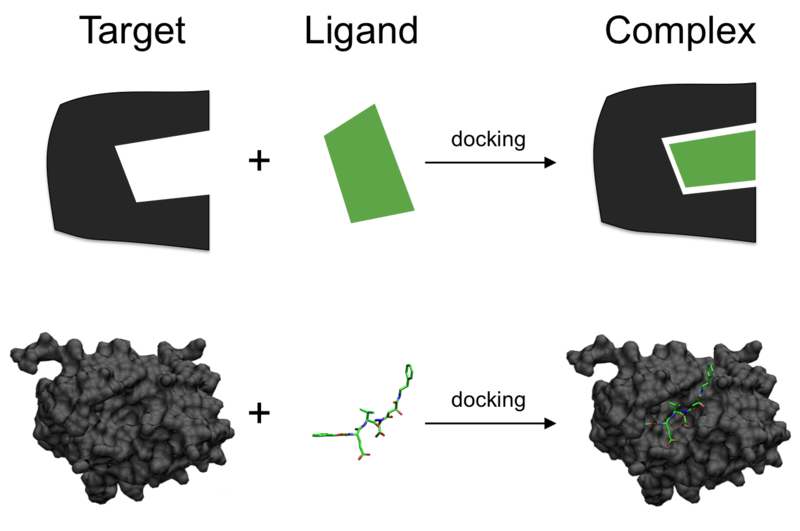
\includegraphics[width=0.5\linewidth]{Docking_representation_2}}
  \caption{Representação gráfica do docking\cite{dockingWiki}.}
  \label{dockGraf}
\end{figure}

\section{Problema}
% Como referimos na secção 1.1 o GPU é uma solução capaz de oferecer grandes aumentos de desempenho na paralelização de partes do processo de protein docking
%
%        O GPU é …… (acho que o texto introdutório da secção 2.2 pode vir para qui)
%
 Como foi referido na secção \ref{motif}, o GPU como solução permite um aumento considerável de desempenho na paralelização de etapas constituintes do processo de docking de proteinas. \par
O GPU ( \textit{Graphical Processor Unit}) consiste na unidade de processamento gráfico existente na placa gráfica instalada em qualquer computador, sendo especializada em processamento gráfico, mais precisamente renderização de gráficos 3D.
 No entanto o GPU também é adequado para processamentos alternativos, que, tal como a rederização de gráficos 3D, são igualmente intensivos demais para o CPU. Na actualidade os GPUs oferecem suporte para interfaces de programação e linguagem de alto nível sendo possivel a quem recorra à execução de um programa no GPU alcançar valores de \textit{speedup} superiores em relação a uma implementação para CPU optimizada. O uso do GPU para este tipo de processamentos é referido como \textit{General-purpose computation on graphics processing units} (GPGPU)\cite{gpgpu}. Exemplos de aplicações podem variar deste cálculo financeiro até aplicações bio-informáticas, como é o caso do docking. É possivel encontrar um panorama detalhado sobre as aplicações da computação de alta performance, sobre forma de catálogo, em \cite{cudaIntro}. Algumas das aplicações presentes no catalogo referido são mencionadas na secção \ref{gpus1}. 
 %        existem já implementações em GPU que usam FFT, mas estas têm a limitação de …
 Existem programas implementados para GPU que recorrem a métodos de correção de matrizes por Fast-Fourier Transform. Neste caso uma das opções a adoptar para optimizações consiste em recorrer a bibliotecas externas especializadas em acelerar as etapas relacionadas com FFT, pois a maior parte do tempo de execução de um docking que use FFT é gasto nestas etapas\cite{piper2014gpu} \cite{shimoda2015protein}, o que faz com que a performance destes programas dependa da eficiência da biblioteca. No entanto o BiGGER, por não utilizar FFT na correlação das grelhas, não necessitará de tais bibliotecas para a versão acelerada por GPU, pelo que a performance desta versão será dependente apenas da implementação em si.
%
%        o BiGGER ...     


\section{Solução}
%  BiGGER em GPU
%        o que é que vais fazer (não como)
Assumindo que a preparação tem condições para avançar para a fase de elaboração, é pretendido implementar a aceleração do algoritmo BiGGER, executando este no GPU. Esta aceleração terá de trazer à versão futura do BiGGER ganhos de speedup consideráveis em relação à versão actual que neste momento recorre apenas ao CPU. 

 \section{Contribuições}
% no fim da tese o que é que fica: identificação das partes do bigger que devem/podem ser executadas no GPU, implementação em GPU dessas computações, avaliação de desempenho
No final da tese, terão sido feitas contribuições para identificar as regiões de código do BiGGER que necessitam de ser executadas no GPU, assim como as respetivas implementações e análise ao desempenho. O código poderá desenvolvido de forma a que possam ser aplicadas manutenções. O produto final será uma versão do BiGGER que garanta uma alternativa mais eficiente em termos de computação e tempo de execução face aos restantes algoritmos de docking de proteinas.

\section{Estrutura deste documento}
O presente documento de preparação assume três capítulos:
\begin{enumerate}
\item{Introdução}
\item{Estado da arte}
\item{Plano de trabalho}
\end{enumerate}
O capítulo \ref{cap1} é feita a uma introdução sobre os conceitos de docking a ter em conta assim como uma formulação do problema computacional associado ao mesmo. No capítulo \ref{cap2} é feita uma visão geral em relação aos diversos métodos e ferramentas de docking, inclusive o BiGGER, indicando as diferenças em relação a este último. Estas ferramentas surgiram antes de ser considerado o GPU para acelerar o docking. Neste capítulo também está incluido uma secção em que são abordados os conceitos associados ao GPU e respetiva programação, assim como o que é que existe em termos de software especifico para docking com acelerações em GPU relacionado com o BiGGER. Como foi implementada essa aceleração e de que forma é que é util para as optimizações a desenvolver para o BiGGER. Também são abordados duas APIs para programação em GPU: CUDA e OpenCL.
Por fim no capítulo \ref{cha3}, é descrito o estado de performance da versão actual do BiGGER, através dos resultados do profiling feito a este. Estes resultados permitem definir as zonas de código do programa que precisam de ser acelerados por GPU e por consequência o plano de trabalho para os acelerar. Aborda-se ainda duas possiveis ramificações sobre como implementar os mecanismos de aceleração ao BiGGER assim como os aspetos positivos e os negativos de ambas. 


%\begin{quotation}
%  \itshape
%  This work is licensed under the Creative Commons Attribution-NonCommercial~4.0 International License.
%  To view a copy of this license, visit \url{http://creativecommons.org/licenses/by-nc/4.0/}.
%\end{quotation}


%\section{A Bit of History} % (fold)
%\label{sec:a_bit_of_history}
%
%The \novathesis\ was originally developed to help MSc and PhD students of the Computer Science and Engineering Department of the Faculty of Sciences and Technology of NOVA University of Lisbon (DI-FCT-NOVA) to write their thesis and dissertations Using \LaTeX.
%%
%These student can easily cope with \LaTeX\ by themselves, and the only need some help in the bootstrap process to make their life easier.
%
%However, as the template spread out among the students from other degrees at FCT-NOVA, the demand for am easier-to-use template as grown.
%%
%And the template in its current shape aims at answering the expectations of those that, although they are not familiar with programming nor with markup languages, so still feel brave enough to give \LaTeX\ a try and rejoice with the beauty of the texts typeset by this system.
% 
%% section a_bit_of_history (end)
%
%
%\section{Disclaimer} % (fold)
%\label{sec:disclaimer}
%
%It is up to you, the student, to read the FCT and/or NOVA regulations on how to format and submit your MSc or PhD dissertation.  
%
%This template is endorsed by the FCT-NOVA and even linked from its web pages, but it is not an official template.
%%
%This template exists to make your life easier, but in the end of the line you are accountable for both the looks and the contents of the document you submit as your dissertation.

